\subsection{Underwater docking: motivation and phases}

Autonomous Underwater Vehicle (AUV) docking has been a focus of research for decades, driven by the need for long-duration missions via subsea battery recharging and data transfer. A wide range of docking guidance strategies has been explored, as summarized in recent surveys \cite{yazdani2020survey}. Broadly, approaches are categorised by the sensing and guidance modality. Acoustic homing using sonar beacons can guide AUVs from long range, often providing range and bearing to a dock \cite{maire2009vision}. Electromagnetic docking systems have also been tested (e.g. using low-frequency EM fields for short-range homing), notably in Feezor's EM homing system \cite{feezor2001autonomous}. Vision-based techniques, using cameras to detect visual markers, offer high precision in final alignment. In practice, multi-modal solutions are common, where for example an AUV might navigate toward a dock via acoustic homing signals and then switch to vision-based guidance in the final meters \cite{maire2009vision}. Dedicated docking markers can be active (such as flashing lights or LED beacons) to increase visibility, or passive high-contrast patterns that require no power, as demonstrated in Maire's pole design. On the mechanical side, most docking station designs incorporate funnel-shaped guide surfaces to help capture the vehicle despite some misalignment. This combination of sensor guidance and mechanical alignment ensures a robust docking process under various conditions.

Numerous projects have demonstrated AUV docking with different infrastructures and homing strategies. One of the earliest was the WHOI REMUS AUV docking system from the late 1990s, which used a Relative Acoustic Tracking system of acoustic transponders for homing into a funnel-like subsea dock (see Figure~\ref{fig:remus-auv}) \cite{stokey1997docking, 4099107}.

\begin{figure}[H]
    \centering
    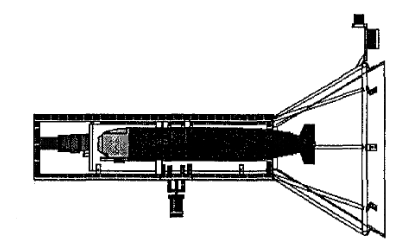
\includegraphics[width=0.6\textwidth]{Figures/remus-auv.png}
    \caption{A side-view drawing of the WHOI REMUS AUV docking system \cite{stokey1997docking}.}
    \label{fig:remus-auv}
\end{figure}

\noindent Researchers have since tested seabed-mounted and moored docking stations to support AUV missions. For instance, Maire et al. (2009) proposed a heavy weighted docking target pole lowered to the seafloor, equipped with an acoustic beacon for long-range localisation and a visual pattern for final approach. An AUV can home to such a seafloor station, attach itself, and enter a sleep or recharge mode until the next mission window \cite{maire2009vision}.

\begin{figure}[H]
    \centering
    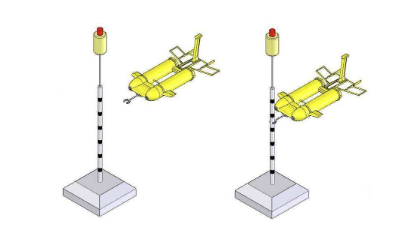
\includegraphics[width=0.6\textwidth]{Figures/maire-dock-diagram.png}
    \caption{Maire et al.'s seabed docking station concept with acoustic and visual homing aids. (left: on approach, right: after docking) \cite{maire2009vision}}
    \label{fig:maire-dock}
\end{figure}

\noindent Remotely operated vehicles (ROVs), being tethered and human piloted, traditionally dock via their tether management system (TMS), a cage lowered from the surface into which a pilot must manually fly the vehicle. Trslic et al.\ demonstrated the first autonomous TMS docking of a heavy work-class ROV in open ocean conditions, using vision-based pose estimation of the four active light markers on a conventional TMS cage (Figure~\ref{fig:trslic-cage}). The trials demonstrated repeated autonomous dockings to the suspended, heaving cage in January North Atlantic sea conditions \cite{trslic2020vision}.

\begin{figure}[H]
    \centering
    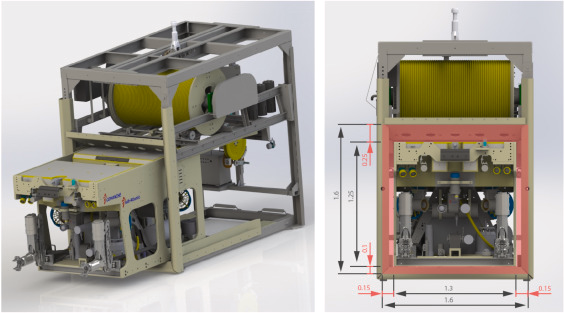
\includegraphics[width=0.6\textwidth]{Figures/trslic-dock-cage.png}
    \caption{The tether management system docking cage for work-class ROVs used in the first autonomous TMS docking demonstration \cite{trslic2020vision}.}
    \label{fig:trslic-cage}
\end{figure}

\noindent In a different configuration, researchers have also developed hybrid docking setups where an ROV acts as a mobile docking station to service AUVs. Morinaga et al.'s docking station ROV captures an AUV using electromagnets, and a slider device then aligns the receiving and transmitting antennas for inductive power transfer (see Figure~\ref{fig:morinaga-auv-flow}). The concept was demonstrated in a water tank docking test \cite{morinaga2021development}.

\begin{figure}[H]
    \centering
    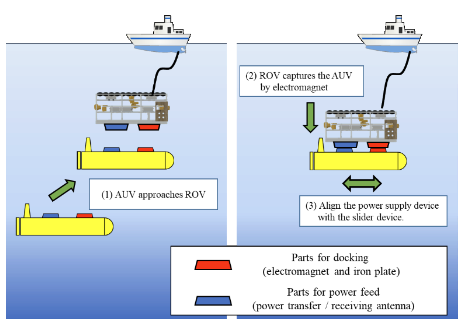
\includegraphics[width=0.6\textwidth]{Figures/morinaga-auv-flow.png}

    \caption{A flowchart of ROV-AUV docking interaction from Morinaga et al. \cite{morinaga2021development}}
    \label{fig:morinaga-auv-flow}
\end{figure}

This illustrates the breadth of ROV-involved docking solutions, from launch and recovery systems to ROVs serving as docking stations for AUV support. Across these systems, the common structure is a two-phase mission, in which long-range homing is followed by short-range terminal alignment. This thesis addresses the terminal phase.
